\documentclass{article}

\usepackage[margin = 3cm]{geometry}
\usepackage[table]{xcolor}
\usepackage{graphicx}
\usepackage{hyperref}
\usepackage{listings}
\usepackage{color}

\definecolor{codegray}{gray}{0.9}
\definecolor{mygreen}{rgb}{0,0.6,0}
\definecolor{mygray}{rgb}{0.5,0.5,0.5}
\definecolor{mymauve}{rgb}{0.58,0,0.82}

\lstset{ 
  backgroundcolor=\color{white},   % choose the background color; you must add \usepackage{color} or \usepackage{xcolor}; should come as last argument
  basicstyle=\footnotesize,        % the size of the fonts that are used for the code
  breakatwhitespace=false,         % sets if automatic breaks should only happen at whitespace
  breaklines=true,                 % sets automatic line breaking
  captionpos=b,                    % sets the caption-position to bottom
  commentstyle=\color{mygreen},    % comment style
  deletekeywords={...},            % if you want to delete keywords from the given language
  escapeinside={\%*}{*)},          % if you want to add LaTeX within your code
  extendedchars=true,              % lets you use non-ASCII characters; for 8-bits encodings only, does not work with UTF-8
  firstnumber=1000,                % start line enumeration with line 1000
  frame=single,	                   % adds a frame around the code
  keepspaces=true,                 % keeps spaces in text, useful for keeping indentation of code (possibly needs columns=flexible)
  keywordstyle=\color{blue},       % keyword style
  language=Octave,                 % the language of the code
  morekeywords={*,...},            % if you want to add more keywords to the set
  numbers=left,                    % where to put the line-numbers; possible values are (none, left, right)
  numbersep=5pt,                   % how far the line-numbers are from the code
  numberstyle=\tiny\color{mygray}, % the style that is used for the line-numbers
  rulecolor=\color{black},         % if not set, the frame-color may be changed on line-breaks within not-black text (e.g. comments (green here))
  showspaces=false,                % show spaces everywhere adding particular underscores; it overrides 'showstringspaces'
  showstringspaces=false,          % underline spaces within strings only
  showtabs=false,                  % show tabs within strings adding particular underscores
  stepnumber=2,                    % the step between two line-numbers. If it's 1, each line will be numbered
  stringstyle=\color{mymauve},     % string literal style
  tabsize=2,	                   % sets default tabsize to 2 spaces
  title=\lstname                   % show the filename of files included with \lstinputlisting; also try caption instead of title
}

\newcommand{\type}[1]{\smash{\colorbox{codegray}{\texttt{#1}}}}
\graphicspath{ {./Images/} }


\title{Accelerating Structural Sum Types}
\author{Luuk de Graaf}
\date{December 2023}

\begin{document}

\maketitle

\tableofcontents

\newpage

\section{Introduction}

Abstractions in programming languages simplify code and allow for implicit exploitation of arising properties.
Pure functional array languages utilize the independence between computations to implicitly parallelize array operations.
This is complicated in languages that are not inherently thread-safe.
Many high-performance applications adopt a data-oriented design, which centres around data transformations and avoiding abstractions around data. 
Both parallelization opportunities and cache efficiency are focal points of the data-oriented design paradigm.
A challenge with data-oriented design is representing non-uniform data efficiently while preserving vectorization opportunities and type safety. 
The issue can be illustrated through raytracing, an embarrassingly parallel problem with several instances of iterating on non-uniform data.

\begin{verbatim}
    image that explains raytracing
\end{verbatim}

An instance of iterating on non-uniform data is the recursive case of a ray intersecting with geometry.
The exception state of a ray not intersection with any geometry is propagated along, which prevents any vectorization attempts of subsequent rays. 
In practice this is solved by either unconditionally executing subsequent rays or eliminating all failure states for each recursive step.
Conditionally throwing the exception can also be redundant when the identity of the variant is inherit to the value, such as a negative distance in intersection algorithms. 
Some raytracers also support geometry shapes outside triangles, such as spheres.
Intersection of multiple shapes can be done within the same function, or by treating all shapes separately.
These approaches are all similar in intent\footnote{This is not necessarily semantics, as unconditional execution can have (acceptable) side-effects in some instances.}, to iterate on a specific variant of a type, but can have significant runtime performance implications.

\begin{verbatim}
    show intent of a function

    constructor

    deconstructor
\end{verbatim}

An efficient and type-safe abstraction is non-trivial as value-level variants and type-level variants exist separately in many languages.  
Unification of these concepts reformulates operating on non-uniform data to an optimization problem.

Operating on multiple variants of a type can be done on the type-level or on the value-level.
In the context of iterating on a collection of variants, branching on a value tag or dynamically dispatching will inherently break vectorization.
This means static polymorphism is a common way to operate on non-uniform data in data-parallel applications.
In some cases this is impossible as the identity of a variant will only be known at runtime, such as exception states but also diverging states.
Conceptually both approaches serve the same purpose, granting the ability to operate on multiple variants of a type.
Unification of these concepts reformulates operating on non-uniform data to an optimization problem.

A type-safe way to achieve this is by elevating the concept of a mutual exclusive datatype to the type-level.
This can be achieved through type-level constructors and datatype-generic functions.
Such implementation can exist without it being natively supported as construct in the implementation language.
This can be utilized by libraries, frameworks and embedded domain-specific languages that exist in languages that facilitate type-level programming, like Haskell.

\newpage

\subsection{Related Work}

The contribution can be categorized as an interdisciplinary between three distinct fields.
Initial objective was establishing computationally efficient representations for non-uniform data in data-parallel applications.
This induced the need for a flexible and type-safe interface, which has been achieved through type-level and datatype generic programming.
Relevance is established through an implementation in a data-parallel language embedded within Haskell.

\paragraph{Representation}

The memory representation of a datatype is often based on the functionality they perform within a language.
In data-parallel applications primitive types are distributed over multiple arrays to facilitate vectorization.
It is not apparent what the representation of a tagged union should be, as they inherently break vectorization in most cases. 
The functional data-parallel languages Accelerate\cite{accelerate-sum-types} and Futhark\cite{futhark-sum-types} implicitly distribute primitive types in composite datatypes over multiple arrays.
Both implementations have limited deduplication capabilities, but research has been done to integrate a memory efficient tagged union in Accelerate\cite{accelerate-sum-types}.
Game-engines, which deal with many clusters of data, have a fundamentally different approach as they have widely adopted the Entity-Component-System (ECS) pattern. 
Many implementations incite a collective re-organization of the internal representation when a variant change occurs at runtime.
A type-safe and performant implementation is notably hard due to having to statically resolve all interactions between the representations, which means meta-programming and untyped code are extremely prevalent. 

\paragraph{Type Interface}

Functional languages handle tagged unions safely through Algebraic Data Types (ADTs), where sum types categorize ADTs with multiple variants.
Constructors can be local to an unique ADT (nominally typed) or exist as independent types (structurally typed).
Deconstructing is done by pattern matching, where functions natively branch on the current active variant.
In Haskell sum types are nominally typed, which means variants are not standalone types and cannot exist safely outside the ADT.
Structural sum types are often called extensible or open sum types, as they do not have to be explicitly declared before use.
In OCaml these are natively supported as polymorphic variants, while Haskell libraries such as {\it fastsum} or {\it extensible} implement them through the type system.
An efficient internal representation can be derived statically through associated types\cite{associated-types}.
Datatype generic functions, which depend on the structure of a datatype, can be used to create isomorphic mappings between representations.
Both concepts are used in highly generic libraries for a wide-range of applications\cite{generic-programming}. 

\paragraph{Implementation}

Libraries and domain-specific languages that are embedded construct their user-defined-types through the host-language.
A shallow embedding operates directly on types native to the host-language, while deep embeddings construct an abstract syntax tree that is later evaluated.
The latter offers flexibility on how user-defined types are implemented, as types exist both on the surface level and as construct within the abstract syntax tree.   
There are several approaches, which have been subject to research in the domain of circuit design.
\begin{itemize}
    \setlength\itemsep{0em}
    \item {C$\lambda$aSH} is not deeply embedded and operates on user-defined types through generics\cite{clash}. 
    \item Hydra has the deep embedding constructs nested into the shallow embedding constructs\cite{hydra}.
    \item Kansas Lava has both embeddings exist in parallel under an encasing type\cite{kansas-lava}.
    \item ForSyDe has both embeddings exist as standalone types\cite{forsyde}.
\end{itemize}

An observation is that user extendability is limited on deeply embedded constructs as execution models must be updated.
A proposed approach is to have a small deeply embedded core language that only supports constructs that are relevant for combinatorial optimizations\cite{shallow-and-deep}. 
The shallow embedding can be used to create an extensible and user-friendly interface to this core language.
In the context of data-parallel applications and non-uniform data this leans itself to an implementation in the host-language.

\newpage

\section{Performance}

There are many components that can influence the performance of a program.
This grows the importance of being able to identify {\it bottlenecks} but also understanding the underlying technological performance considerations\cite{programming-optimization}.
Within the first section fundamental optimizations related to the interaction between data and hardware are introduced.
This is used to identify architecture agnostic performance considerations for array operations in the second section.

\subsection{Optimizations}

In the early days of computing, memory was seen as a way to store data indefinitely.
As computational power of processors increased, the importance of main memory increased.
Main memory is dependant on the advancements of random-access-memory (RAM), which stagnated due to both cost and physical limitations\cite{memory}. 
This put pressure on the software side to adapt to hardware components for optimizations, rather than merely the computational complexity of algorithms.

\begin{figure}[ht]
    \centering
    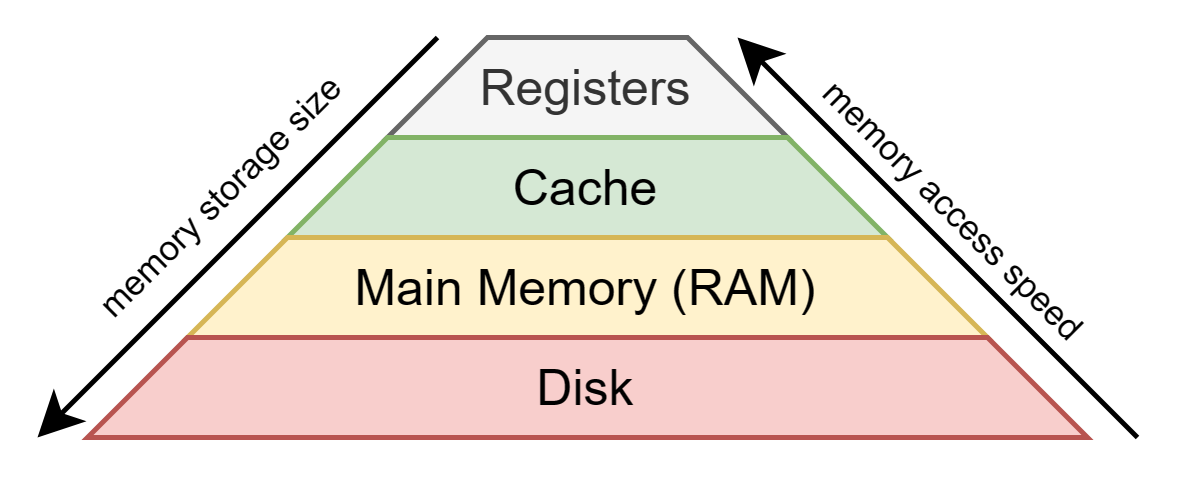
\includegraphics[scale=0.2]{memoryhierarchy}
    \caption{ memory hierarchy }
\end{figure}

One of these hardware optimizations is cache storage, which accelerates memory accesses of predetermined data.
The data is decided based on a cache replacement policy, often based on a temporal property. 
The cache operates independently of the operating system\cite{memory}, and no direct control can be exercised.

\paragraph{Instructions}

Interfacing with processors is done through computer instructions.
Fetching of an instruction is a memory operation, as it retrieves the instruction at the target of the program counter.
Instructions operate on registers, which have distinct sizes depending on the architecture and their respective function.
There are many instruction set architectures (ISA) and devices that implement distinct instruction sets.
An intermediate representation (IR), such as the LLVM IR\cite{LLVM}, can be used to create a uniform interface between these instruction sets\cite{intermediate-representation}.
Explicit use of these architecture exclusive instructions can be achieved through compiler intrinsics.
Hardware design sometimes allows for executing specialized instructions\footnote{Note that the term {\it complex instruction} is avoided, as this concerns a compact {\it representation} of several instructions. }, which are faster than their semantically equivalent instruction(s).
This includes sacrificing accuracy for performance (floating-point), combining a sequence of instructions (arithmetic) or by parallel execution on multiple data elements (SIMD).
SIMD instructions in particular are often very performant, as several steps within the execution pipeline can be parallelized.
This process of instruction parallelization is called {\it vectorization}.

\begin{figure}[ht]
    \centering
    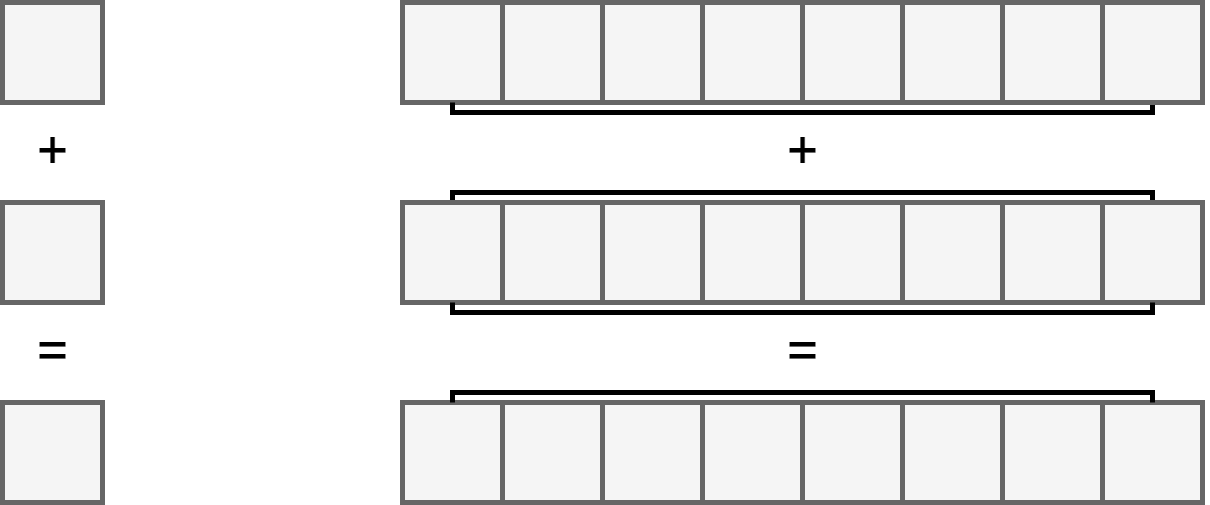
\includegraphics[scale=0.2]{vectorization}
    \caption{ vectorization of a scalar addition operation }
\end{figure}

\newpage

\paragraph{Register Pressure} 

Registers can be considered the fastest available memory, as the data is ready to be used by an instruction.
Within the context of registers this data is commonly referred to as a variable.
Variables existing within registers before execution is a prerequisite for reasonable performance.
This scheduling problem is to be considered a NP-complete problem\cite{register-allocation}.
Programming languages with any form of abstraction delegate this process to the compiler.
This simplifies a lot of complexity, as only which data is being used by what instruction is relevant.
In some cases there are too many live variables for the available registers, which {\it spills} the variable.
This requires a variable to be stored outside registers, in a slower form of memory, and incites a delay upon use.
This can be prevented by reducing the live-time of variables, reordering instructions and diversifying execution units.  

\paragraph{Memory Access Time}

Semantically random-access-memory (RAM) implies that memory operations take around the same amount of time.
In practice this does not hold for several reasons.

\begin{itemize}
    \item [SRAM/DRAM]
    On a modern system there often exist several different types of RAM, mostly driven by cost differences.
    The main forms of RAM are static RAM (SRAM) and dynamic RAM (DRAM).
    SRAM uses six transistors to represent a single bit, while DRAM only uses one transistor with a single capacitor. 
    A capacitor loses electrons over time which means data has to be refreshed repeatedly to preserve its data.
    A refresh requires both read and write operations, which interferes with other memory operations.
    This makes DRAM inconsistent and on average significantly slower but much cheaper to produce due to requiring less transistors.\cite{memory}

    \item [Propagation]
    Data is transferred by using electrical charges through semi-conductors.
    This creates a physical limitation dictated by physical distance and temperature.
    This is called propagation delay and a hard limitation to the rate at which components can operate on.
    SRAM is often located physically closer to the execution units to utilize the faster memory access more effectively.
 
    \item [DMA]
    A processing unit needs to forward the requested data to the targeted location, which takes up processing time.
    Direct-memory-access (DMA) is an interface for hardware components and allows memory operations to be more organized.
    This allows for large scale memory operations to be performed efficiently and independently of the main processor.
    It requires use of several buses which means some processors must idle at seemingly random periods of time.
    This means that other hardware components can influence the memory access time.
 
\end{itemize}

\newpage

\paragraph{Caching}

Due to hardware related discrepancies in memory access time, it can be beneficial to organize data according to the memory access time.
One way to achieve this is by caching data, that is storing a {\it copy} of the data in faster accessible medium.
A cache is generally made of SRAM and resides close to the processor, which allows memory accesses to be magnitudes faster than the equivalent main memory access\cite{memory}.
When data already exist in the cache it is referred to as a {\it cache hit}, otherwise a {\it cache miss}.
Deciding which data is cached and for how long is a cache replacement policy.
Adapting to these policies simplifies the scheduling and minimizes the amount of cache misses.

\begin{figure}[ht]
    \centering
    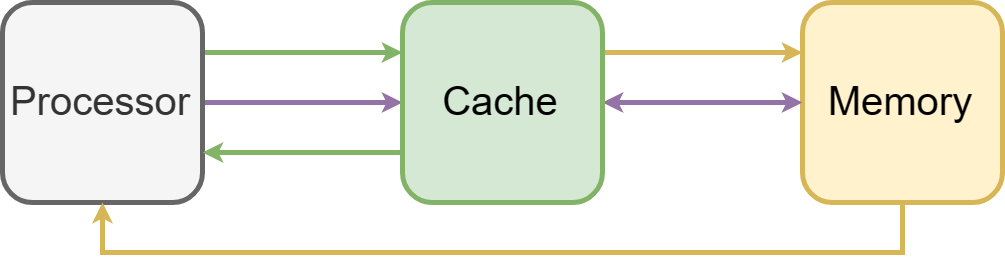
\includegraphics[scale=0.3]{cache}
    \caption{ cache hit (green), cache miss (yellow) and replacement (purple)}
\end{figure}

Caching of data can be done after the data has been retrieved, which means the delay already has occurred.
This can be avoided by requesting data in advance and storing it a cache prematurely, so called cache prefetching.
This is done by analyzing future instructions (hardware) and instructions that {\it hint} at the future use of data (software)\cite{cache-prefetching}.

\begin{figure}[ht]
    \centering
    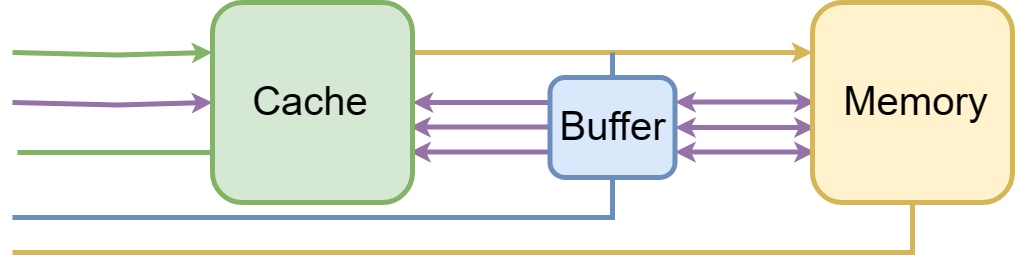
\includegraphics[scale=0.3]{prefetch}
    \caption{ prefetch based on information (blue) from cache miss and processor instructions }
\end{figure}

This is harder when a branch is encountered, as both the data and the next instructions are uncertain.
Speculatively executing these uncertain instructions can be performant if the overhead of redundant work remains small enough.
Rather than executing unconditionally, some processors execute the most likely to happen branch based on some parameters (branch prediction)\cite{instruction-level-parallelism}.
 
\newpage

\paragraph{Parallelism}

Instruction-level parallelism is the parallel execution of multiple instructions\cite{instruction-level-parallelism}.
This can be done by dividing instructions into several steps and outsourcing each step to a distinct processor unit (instruction pipelining).
Shuffling the order of instructions can allow more processor units to work in parallel (out-of-order execution).
Duplicate units and independent instructions allows for additional parallelism (superscalar execution).

\begin{figure}[ht]
    \centering
    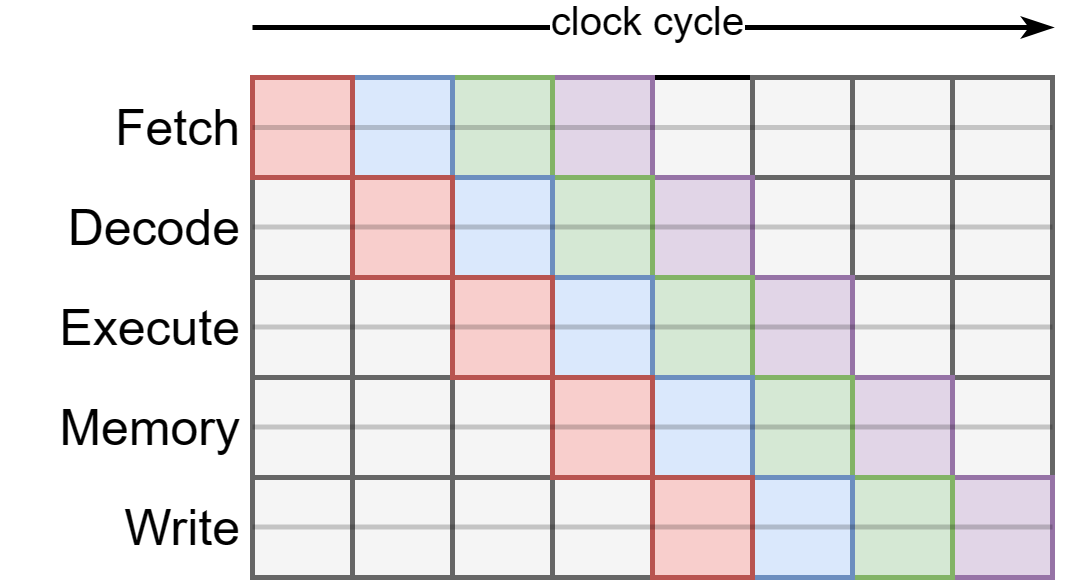
\includegraphics[scale=0.2]{instructionlevelparallelism}
    \caption{ instruction pipelining: each color represents an instruction }
\end{figure}

Data-level parallelism executes an instruction on several data elements, such as the previously discussed SIMD instructions.
Specialized processors sometimes either fully pipeline the data (vector processing) or allow for some form of autonomy (multithreading). 
Both share instruction fetching and decoding, but threads have their own program counter which allows for an independent sequence of instructions.

\begin{figure}[ht]
    \centering
    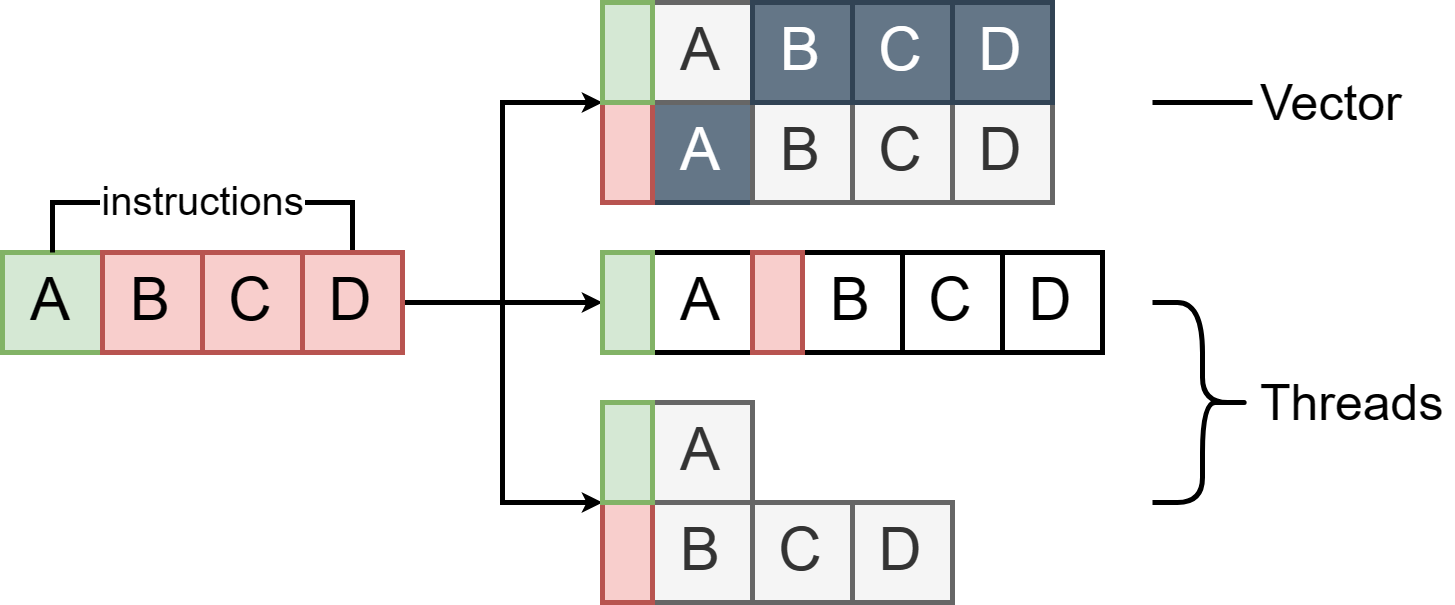
\includegraphics[scale=0.2]{vectorvsthreads}
    \caption{ branch instructions: masking (vector) vs independent sequence (threads)}
\end{figure}

Execution of threads can be done concurrently, which can be useful to hide latencies (context-switching).
In parallel is also possible with multi-core processors, which have several processors units (cores) that can support multiple threads.
Cores are often not independent processors and might share several components with other cores, such as caches\cite{thread-level-parallelism}.

\newpage

\subsection{Principles}

There are many components that can influence the performance of a program, some of which were discussed in previous sections.
This makes general statements on optimizations often weak, as the interaction between these components is complex.
Focusing on a particular area, such as iterating on data elements, allows for stronger arguments.
Within this section previously discussed optimizations will be discussed in the context of iterating on many elements.

\paragraph{Contiguous} 

A rudimentary reason for contiguously allocated data is that it creates structure, which can be used to organize data.
Arrays utilize their structure to align elements, such that each element can be identified in constant time\footnote{Both in {\it time complexity} and within {\it computer architecture} norms, as data access is a single instruction, unlike pointer trees and hash tables. } through a linear function.
This is also used for compound datatypes, where structure and the type can identify the memory location of each field.
The structure also simplifies work distribution between threads, as it is a matter of constant offsets.
For vectorization contiguous data is a prerequisite as instructions operate on singular contiguous blocks of data.
If data is not spatial adjacent in memory, data must aligned temporarily or complex interleaving methods must be used\cite{interleaved-SIMD}.
In the general case compound datatypes interfere with vectorization, as spatial adjacent data is not of the same type.
Parallel arrays solve this by creating a distinct array for each primitive type (Struct of Array) so that each field can be vectorized.

\begin{figure}[ht]
    \centering
    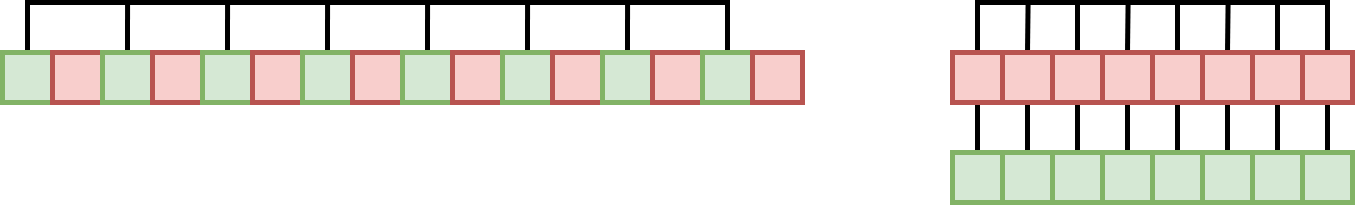
\includegraphics[scale=0.2]{parallelarray}
    \caption{ compound datatype array (1) and a parallel array (2) }
\end{figure}

Caches also operate with contiguous blocks of memory, which means spatial adjacent data within a fixed alignment are stored together.
This lends itself well to contiguous allocated data, as it means the least amount of cache blocks are required irrespective of block size and alignment.
In addition all memory accesses use the same linear function, a {\it constant stride} access behavior, which makes it receptive to hardware cache prefetching\cite{cache-prefetching}. 

\paragraph{Access Patterns}

As the cache is finite a cache block can be ejected prematurely.
This exists for data within the same block but also when the same block is required at multiple times.
Increasing temporal locality is done by avoiding random accesses and organizing computations order around data usage.
This is non-trivial in iterations where multiple indices are accessed (stencils) or computations that inherently involve random access.

\begin{figure}[ht]
    \centering
    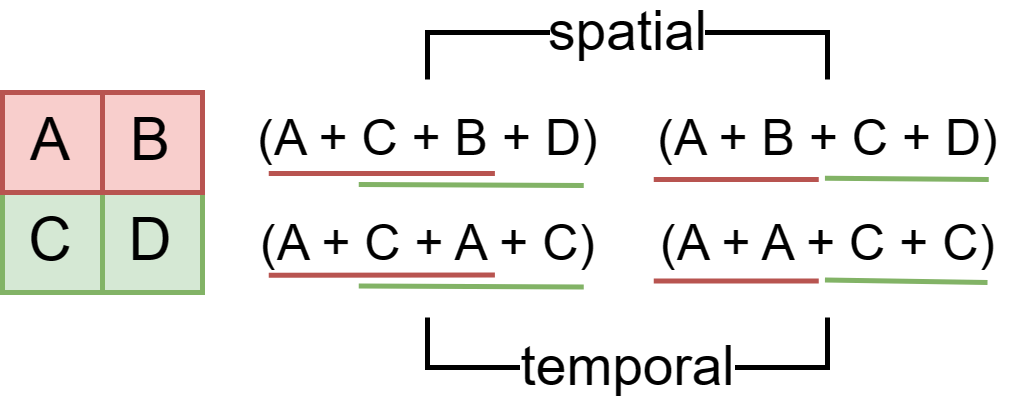
\includegraphics[scale=0.25]{locality}
    \caption{ exploitation of spatial and temporal locality }
\end{figure}

\newpage

One way to apply this to iterating on many elements, is to iterate one subset of elements at a time (tiling).
This can be further improved by also accounting for shared resources, by grouping elements that use the same resource in their instruction sequence. 
This is explored in raytracing\cite{raytracing-reorder-ray}, where spatial locality of rays is used to exploit the cache coherence within the traversal of a tree.
These techniques are also important for multi-core processors, as it reduces the need for data to exist in multiple caches.

\paragraph{Branching}

Pipelining instructions is not possible when the sequence of instructions is dependant on the result of a previous instruction.
This limits instruction-level parallelism, which is solved through various unconditional instruction executions\cite{instruction-level-parallelism}.
Either by discarding the computed results or by {\it flushing} the pipeline when the wrong branch is predicted, both of which intuitively have an overhead.
A compiler can eliminate\footnote{Either by proofing the branch will never be executed or by replacing the branch with a {\it conditional move} instruction, which only writes the result on true.}  branches or move loop-invariant code to facilitate instruction-level parallelism\cite{assembly-optimizations}. 
These optimizations are not absolute, as an increase in instructions can pressure registers and the cache.  
It is also limited to instructions that cannot fail or overflow, as both can introduce unintentional side-effects.  

\begin{figure}[ht]
    \centering
    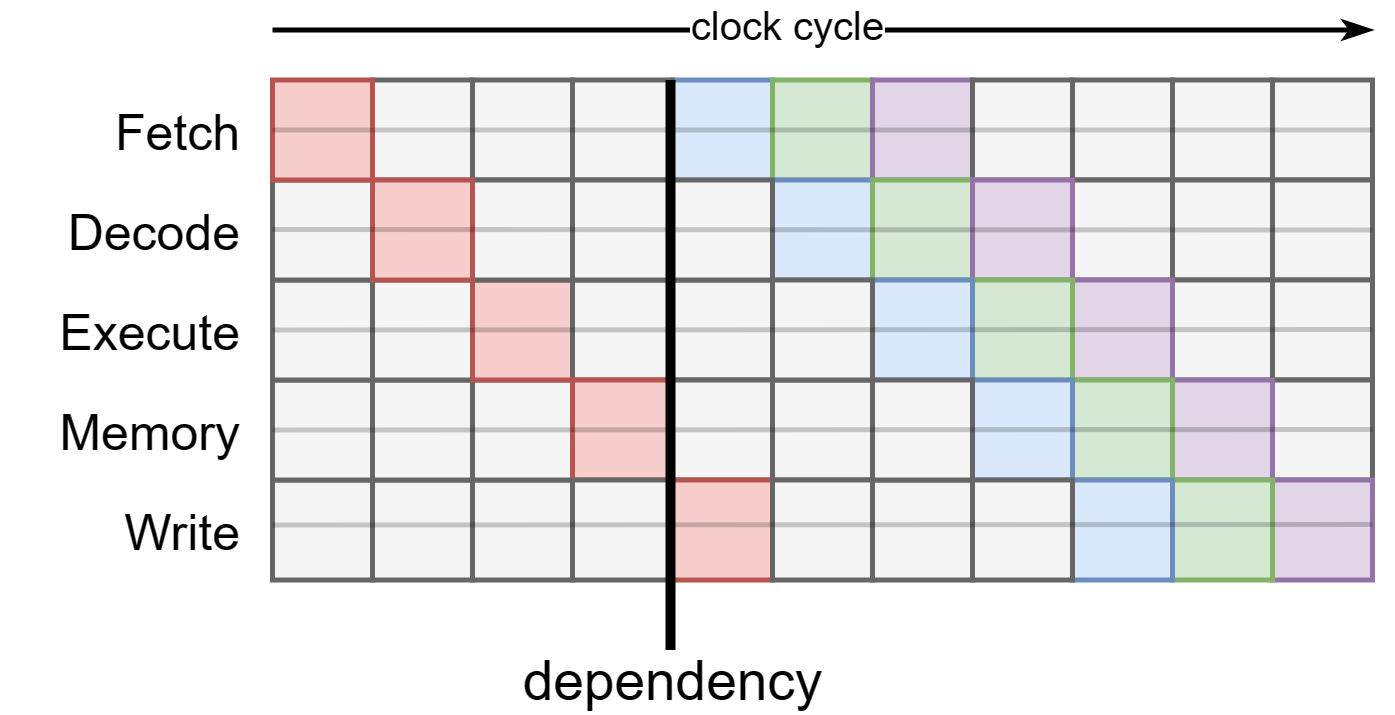
\includegraphics[scale=0.15]{branchcost}
    \caption{ branch introduces dependency on execution of instruction (red) }
\end{figure}

Branching is also problematic for vectorization, as all data within a certain alignment must follow the same sequence of instructions.
This can be resolved through the use of a {\it bitmask}, which can nullify parts of a result\cite{assembly-optimizations}.  
The additional instructions and computing bit masks can prevents performance from vectorization in certain situations.  
A notable application is sequential loops, where unrolling creates an opportunity to vectorize the scalar instructions.
Automatic vectorization is an active field of research, and limitations have been primarily attributed to the lack of analysis information available to compilers\cite{automatic-vectorization}. 
This means branchless code and simplifying control flow allows the compiler to vectorize in more instances.

Specialized processors where an instruction sequence is distributed over many cores are limited to executing all branches.
This is minimized through the use of Streaming Multiprocessors (SM), which contains several cores and fetch their own instructions.
Streaming Multiprocessors operate and schedule warps, which often contain 32 threads.
When divergence between these threads occurs ({\it branch divergence}) the instructions will in the general case be executed in lockstep\cite{threads-independent-scheduling}.

\newpage

\subsection{Data structures}

A fundamental aspect of computing is data structures, which is a constant overhead for all computations.
For collective operations arrays are essential; as they have a constant access time, are contiguously allocated and access can be parallelized.
Composite datatypes within arrays introduce some considerations.
One is the {\it implicit} use of parallel arrays, where each primitive datatype is stored in a distinct array.
This enables vectorization opportunities, but a random access pattern might cause additional cache blocks to be cycled between.
Since collective operations control the access pattern, parallel arrays are often a natural choice for array languages.
The consideration for both structurally and functionally distinct data, now referred to as variant, is often complex.
Variants can be represented on an individual basis (element-wise) or collectively (variant-wise).
Usage and implementations of these approaches are explored in this chapter. 
Within this chapter the assumption is made that parallel arrays are used, as they align with the intention to vectorize operations. 
The example composite datatype has type \textcolor{blue}{A}, and either has type \textcolor{red}{B} or type \textcolor{green}{C}.

\subsubsection{Element-wise}

For each element the choice of variant is represented, which introduces branching and in the general case will break vectorization.
As variants are not grouped, functions cannot iterate on a specific variant without iterating on the complete array.
The main advantage is that a variant change can be done independent of other elements, and thus can be parallelized.
A practical consideration is that each element in an array must be structurally the same, that is they occupy the same memory space.
This is a limitation which enforces that each index can determine the location of an element. 
For parallel arrays this restriction applies for all arrays individually\cite{accelerate-sum-types}.

\paragraph{Tagged Union}

Multiple variants can be represented through a tag and a fixed size data component with multiple representations, so called {\it union}.
The tag is used to identify the current representation of the union. 
A naive implementation creates an array for each field of each variant, which means the memory usage is cumulative for each variant. 
A compact tagged union overlaps fields of variants, as only one representation can be valid at a time.
This can in theory reduce the size to the largest variant and the accompanied tag, but this is complicated due to alignment requirements\cite{accelerate-sum-types}.

\begin{figure}[ht]
    \centering
    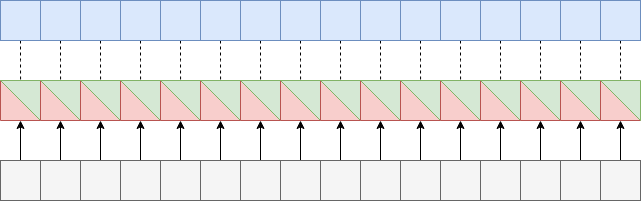
\includegraphics[scale=0.4]{taggedunion}
    \caption{ index implicit and tag (gray) identify the data representation }
\end{figure}

\newpage

\paragraph{Tagged Pointer}

Another way to comply with elements being structurally the same is to use a form of indirection, in this case a pointer to memory.
The indirection allows variants to escape the uniform size restriction, but there are several notable complications.
General complications around pointers, such as being unsafe to operate on and complicating garbage collection apply.
In addition, pointers that point to the same data (alias) can prevent parallelization due to possible race conditions.
These can be partly solved through language constructs; such as smart pointers, immutable data or abstracting the use of pointers altogether.

\begin{figure}[ht]
    \centering
    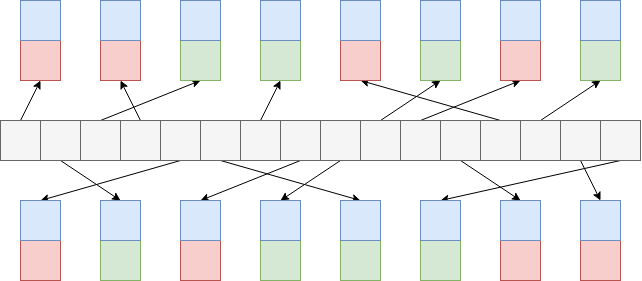
\includegraphics[scale=0.4]{taggedpointer}
    \caption{ tag and pointer (gray) identify the location and representation. }
\end{figure}

The key issue is that a change in variant requires new data to be allocated and the pointer to be adjusted.
This allocation means there is no guarantee that the data is contiguous, which in addition to the required branching prevents any vectorization efforts.
The indirection and fragmented memory is also problematic for cache efficiency, as it is unpredictable and a cache block is not used effectively.

\newpage

\paragraph{Entity}

A notable observation is that the re-allocation of a variant change causes the data to be not contiguous, not the indirection in itself.
This can be illustrated through a hash table data structure, where a key is mapped to a value within an array (bucket).
Any collective operation on the hash table can be vectorized by disregarding the hashing and using the internal array directly, as computations are inherently independent and order is irrelevant.   

\begin{figure}[ht]
    \centering
    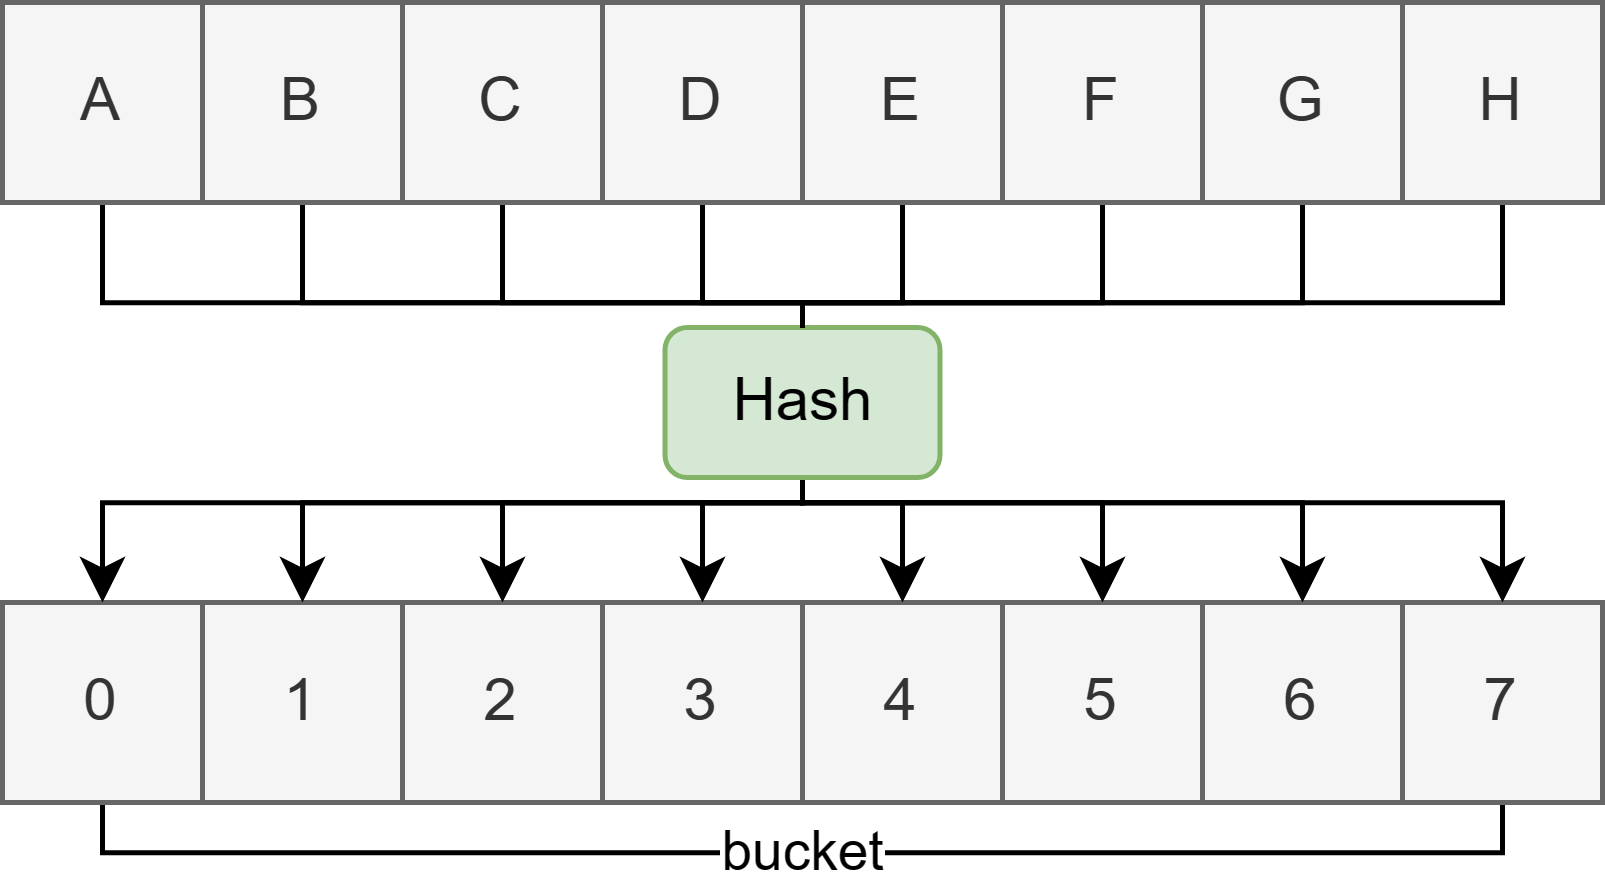
\includegraphics[scale=0.1]{hashtable}
    %\caption{ hash table }
\end{figure}

Entities within the ECS pattern function similarly, a form of indirection that is not used by the collective operations. 
Represented as a single heterogeneous array, which internally consists of several variant-wise collections. 
It will mean that variant choice is not {\it directly} represented on an element basis, which has several implications.

\begin{itemize}
    \item [Stable] 
The same entity is not guaranteed to refer to the same data, the entity is no longer stable across structural changes.
The reverse also holds, the data is not guaranteed to have the same entity along iterations.
This can solved by tracking the location of entities {\it or} annotating the data with their entity. 
These approaches can be complementary for performance reasons, but they are collectively isomorphic\footnote{A single entity cannot identify the data in constant time, without an array of pointers. A data element cannot identify the entity in constant time, without the entity as data. } through gather and scatter operations. 

\begin{figure}[ht]
    \centering
    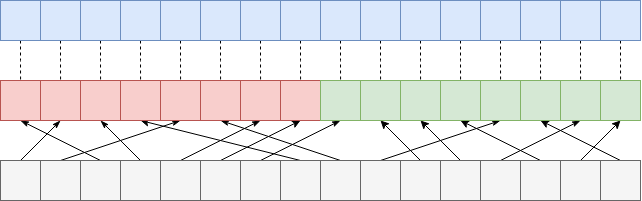
\includegraphics[scale=0.3]{stable1}
    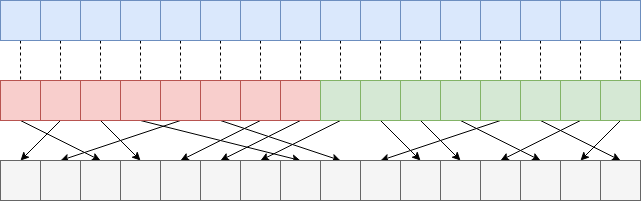
\includegraphics[scale=0.3]{stable2}
    \caption{ persistent array with indirection (1) or annotate the data with their index (2). }
\end{figure}

For many array operations stableness is excessive, as it means data is discriminated on the basis of their index. 
The implicit connection that data with the same index has can be represented through a (temporary) datatype.

    \item [Independent]
Elements can no longer change their variant independently of other elements, which can be problematic for parallelism.
Depending on the way variants are grouped, there can also be a significant cost associated with regrouping variants.
This can be minimized by delaying structural changes indefinitely, by using a tagged union approach.
Regrouping variants is a performance consideration between the cost of regrouping and having to branch for future iterations.
\end{itemize}    

\newpage

\subsubsection{Variant-wise}

Grouping variants means all data is uniform, contiguously allocated and there exist no inherit branching within the same grouping of variants.
This can be achieved through an array for each variant, but also grouping {\it within} the same array and using segment descriptors.
The latter is effectively an untagged union, where the representation is determined by the index within the array.
Both allow instructions to be vectorized, but there exist several other considerations.

\begin{itemize}
    \item [grouping]
    As stated in the previous section, regrouping variants to a variant-wise collection is a performance consideration.
    When variants are stored in separate arrays, the amount of a certain variant must be known before allocation.
    When this is dependant on a computation, it can be retrieved through an additional scan or atomically\footnote{Atomic instructions prevent interruptions by other processes and are thread-safe.} counting any structural change, which adds an overhead.
    This is not required for a singular array if the total remains the same.

    \item [immutable]
    An important consideration for purely functional languages is that values, and therefore arrays, are to be considered immutable.
    This means that {\it{updating}} parts of an array efficiently is non-trivial.
    It must be proven that the array before update will never be used again, otherwise both arrays must co-exist in memory.
    This is inefficient for small updates and grows the necessity to {\it destructively update}\cite{destructive-update-array}.

    \item[automatic]
    Most compilers support automatic vectorization of iterations with flexible bounds, where the final leftover iteration is not vectorized.  
    This overhead can be a significant when the loop is extensively unrolled.
    This is minimized through epilogue vectorization, which (re-)applies loop vectorization to the remaining scalar code.
    In practice data must be aligned along specific byte boundaries to be vectorized, which is challenging for (dynamic) regions within an array and not always analyzed by compilers\cite{automatic-vectorization}.

    \item [operable]
    An undiscussed benefit of parallel arrays is that fields can be operated on independent of other fields, as they are distinct arrays.
    This is also possible for {\it regions} within an array, but this is less trivial and often requires explicit support in array languages\cite{accelerate-independent-regions}. 


\end{itemize}

\begin{figure}[ht]
    \centering
    \includegraphics[scale=0.3]{variant1}
    \hspace{10pt}
    \includegraphics[scale=0.3]{variant2}
    \caption{distinct arrays (1) or distributed in a single array (2)}
\end{figure}

\begin{figure}[ht]
    \centering
    \includegraphics[scale=0.3]{variant3}
    \caption{combination of both approaches}
\end{figure}

\newpage

\subsection{Memory Representation}

Memory instructions operate on fixed boundaries, which means operations that overlap these boundaries require additional but strictly unnecessary instructions.
A natural alignment of a datatype is achieved by aligning all types according to the instructions that access them\footnote{SIMD instructions}. 
Many compilers introduce {\it padding} to enforce natural alignment.
While computational efficient, the alternative of {\it packing} types together can be preferred for a smaller memory footprint.  
Both approaches can be used to ensure the datatypes align with cache lines. 

\begin{figure}[ht]
    \centering
    \caption{data alignment example with cache lines (c++ code)}
\end{figure}

Parallel arrays (Struct of Arrays) have a natural alignment by default as they contain primitives types, which are naturally aligned.
General purpose languages often default to the Array of Struct, while data-parallel applications use the Struct of Arrays representation.
A zero-cost abstraction that can ergonomically switch between these constructs is non-trivial.
An interface to index access with an intermediate structure can break automatic vectorization\cite{abstraction-vectorization}. 
In addition the different internal representations must be statically definable and able to be handled by the data structures.
Many C++ libraries utilize {\it class templates} to achieve this\cite{abstraction-vectorization}.
Being able to switch between representations was an initial focal point of the experimental language {\it Jai}, a c-like programming language for games.
The switch between representations is currently possible through a more general pre-processors macro's approach.

\newpage

\section{Interface}

A preliminary conclusion of the previous chapter is that a performant internal representation cannot be deducted from a mere theoretical framework.
With this in mind it is important for high performance oriented applications to be flexible with the internal representation of datatypes.
This is important for both composite data types and data structures.
Within this chapter a modular interface is explored around iterating on collections of non-uniform data.

\subsection{Paradigm}

As discussed in the data structures section, there are two internal representations for collections of non-uniform data.
Variants of a particular type are stored either element-wise or variant-wise.
There are several considerations for a data structure that is agnostic to if it stores non-uniform data in element-wise or a variant-wise way.
A variant-wise collection can operate on only the relevant variants, while an element-wise is forced to discover that at runtime.
To avoid redundant iterations for variant-wise collections, a function must be able to be defined on the most specific subset of all variants.
For element-wise collection the amount of variants must be finite and no large discrepancies exist between the size of all the variants.

\begin{verbatim}
    image explaining the issues of both cases (maybe use raytracing)







\end{verbatim}

For variant-wise collections the ECS-pattern will be used as reference.
The first section goes into how the ECS-pattern collectively operates on only certain variants.
For element-wise collections Algebraic Data Types (ADTs) are used to safely discriminate between multiple variants as element. 
The second section utilizes structurally typed ADTs to create an efficient interface for a variant-wise and element-wise collection.  

\newpage

\subsubsection{Entity-Component-System}

The ECS pattern is arguably a reaction to the prevalence of object-oriented languages within game engines.
The premise is to organizes game-logic within functions rather than data, where the relation between data is flexible\cite{ecs-origin}.
In contrast to inheritance, where relations are statically determined and game-logic is embedded within an predetermined hierarchy.
The pattern is often combined with data-oriented design and is used to be able to implicitly exploit data-parallelism in general purpose languages. 
While there exist many implementations of the pattern in many languages, the principles remain similar.  

\paragraph{Components}
A component is the smallest addressable type within the pattern.
Examples of components are \type{Position} and \type{Velocity}, which together represent movement.
Components are generally value types to avoid race conditions when using data-parallelism.
Some implementations allow for a (readonly) reference component that is shared along multiple instances.
A shared \type{Mesh} component prevents redundant geometry to be stored by referencing it.

\paragraph{Entity}
An entity is idiomatically a set of components.
A movable entity has the \type{Position} and \type{Velocity} components, while an immovable entity only has the \type{Position} component.
Adding and removing components is done at runtime and there is no predetermined relation between any of the components.   
Any immovable entity can be made movable by attaching the \type{Velocity} component at runtime.

\paragraph{Systems}
A system operates on all entities that match a specific set of components.
The \type{Movement} system will operate on all movable entities, irrespective of any other attached components.
Systems are effectively global functions, which operate only on specific variants of the more general entity type. 
This allows for a variant-wise collection of entities, which most ECS implementations enforce to implicitly create performant vectorized code.

\begin{figure}[ht]
    \centering
    \includegraphics[scale=0.2]{ecs}
    \caption{ conceptual entity-component-system representation of systems }
\end{figure}

The ECS design pattern is arguably inherently imperative, as structural changes to entities are done imperatively.
Apecs, an ECS library in Haskell, achieves this imperative style through monads\cite{ecs-apecs}.
The ECS pattern makes element-wise collections infeasible, as there is no type-safe way to restrict the possible amount of structural changes to an entity.
This is inherit to the pattern, as any component can be attached to any entity.
Implementations circumvent this limitation by allowing components to be enabled and disabled through a tag.
Disabling a component changes the {\it type} of an entity but the internal representation remains the same.
An analogy can be made to a non-deduplicated tagged union that is explicit in the variants it holds.

\newpage

\subsubsection{Algebraic Data Type}

Functional languages handle tagged unions safely through algebraic data types (ADTs).
A product type (x) is the combination of datatypes, while a sum type (+) is the alternation between datatypes.
It is often useful to discriminate between variations of a datatype, which is generally done through a data constructor. 

\begin{verbatim}
    
    data Maybe a = Just a | Nothing
    
\end{verbatim}

Deconstructing an algebraic data type is done by pattern matching on a data constructor.
The pattern match can exhaustively match on all variants, as the data constructors of variants are known at compile-time.
It can be seen as a native control-flow mechanism that ensures only the operations on the active variant are applied.

\begin{verbatim}
    
    fmap :: (a -> b) -> Maybe a -> Maybe b
    fmap f (Just a) = Just (f a)
    fmap f Nothing  = Nothing
    
\end{verbatim}

In Haskell, algebraic data types are distinguishable by name (nominally typed) and therefore explicitly declared.
This means data constructors are local to the declared type and pattern matching happens within the same type.
The type signature of the \type{fmap} function provides no information on the potential structural change of a datatype.
It is possible to return \type{Nothing} for both cases\footnote{\type{Just b} is not possible as it can only be inferred through \type{Just a} and the \type{a -> b} function.}.
A function that takes \type{Just a} and returns \type{Just b} ensures that the {\it collective identity} is preserved in a collective operation, irrespective of the data transformation.
This exact definition is not possible due to being nominally typed, as \type{Just a} is not a type but a data constructor under the type \type{Maybe a}. 
In some cases, such as a safe division function, the introduced branching is inherit to the function and is now made explicit in the type definition.   

\begin{verbatim}

    fmap :: (a -> b) -> Just a -> Just b
    fmap f (Just a) = Just (f a)

    divide :: Int -> Int -> (Just Int | Nothing)
    divide _ 0 = Nothing
    divide n m = Just (n `div` m)
    
\end{verbatim}

In this case a function is defined on the structure of a type, the data constructor of algebraic data types.
\type{Maybe a} is now an alias for the mutually exclusive relationship \type{Just a | Nothing}, rather than a unique and standalone type. 
This generalizes variance to be between all types.
OCaml calls these {\it polymorphic variants}\footnote{OCaml also implements nominally typed sum types, so called {\it variants}.}, while other functional languages generally refer to them as {\it extensible} or {\it open sum types}.
A motivating example is that a collection of \type{Maybe a} can be an element-wise collection or two variant-wise collections of \type{Just a} and \type{Nothing}\footnote{As \type{Nothing} does not hold data, a size descriptor is sufficient.}.
While the former involves branching for \type{fmap}, the latter can ignore the \type{Nothing} collection and vectorize the \type{fmap} function.
This flexibility aligns with the intention to create a modular system that is agnostic to the internal representation.

\newpage

\subsection{Type-level programming}

In the previous section an interface that is agnostic to the variant-wise and element-wise collection is proposed.
This demands defining efficient intermediate internal representations for all possible variant combinations, which defeats the purpose of ergonomic switching between representations.
Statically deriving an internal representation is impossible or restricted to predetermined parameters in most languages.
Some high-performance libraries circumvent this restriction by meta-programming or custom data layouts\cite{llama}.
A customizable and type-safe solution is type-level programming, which will be explored in this chapter.

\subsubsection{Kinds}

A value is categorized by types, while a type is categorized by {\it kinds}.
This is relevant when discussing type constructors, where each constructor with a different arity has a distinguishable kind.
A well known exposition of type constructors are parametric polymorphic data types, which take type variables as argument.
While a lot of languages support polymorphic data types, the concept of kinds is not evident as only concrete types are able to be used for arguments.
Haskell supports higher-kinded types, which are analogous to higher-order functions for types, which makes kinds apparent to the user.

\begin{verbatim}
    2.5f         :: Float
    Float        :: *
    Option a     :: * -> *
    Option Float :: *
    Apply f x    :: (* -> *) -> * -> *
\end{verbatim}

Type constructors can be used to encode data statically, such as Peano numbers.
The parametric \type{Succ a} and \type{Nil} types are axioms that can be used to construct a natural number on the type-level.
By default these exist in a open universe, which means ill-formed expressions can be created.
On the type-level this can be resolved by Generalized Algebraic Data Types (GADTs), implemented in Haskell as an extension.
It allows the type variables of constructors to diverge from the more general type.

\begin{verbatim}
    // open universe where 'a' can be anything
    data Succ a
    data Nil

    // closed universe under the phantom type 'a'
    data Natural a where
        Succ :: Natural b -> Natural (Natural b)
        Nil  :: Natural ()
\end{verbatim}

The consequence is that deconstructing a GADT will refine the type.
This can be used to construct evidence of certain properties by pattern matching on data constructors.
An observation is that this is a categorization of types, similar to how the kind \type{*} represents all concrete types.
The \type{DataKind} extension promote types to the kind-level and constructors to the type-level. 
The kind \type{Natural} includes the types \type{Succ (a :: Natural)} and \type{Nil}.
It both creates a closed universe and allows other type constructors to expect the more precise kind \type{Natural}.
A limitation is that the construction of the type, which is needed for arithmetic operations, is guarded by the definition of \type{Natural}.

\begin{verbatim}
    data Natural = Succ Natural | Nil | Add Natural Natural | Minus Natural Natural
\end{verbatim}

On the value-level this is solved through functions that transform their input into another output type.
Translated to the type-level it means type-level functions that transform an input kind into an output kind.

\newpage

\subsubsection{Type Family}

A way to approach type-level functions is to see it as a type dependent on the instantiation of a type variable.
This is akin to functions in type classes, where type-indexing allows functions to be overloaded.
Haskell reuses this functionality for types, categorizable as {\it associated types}\cite{associated-types}.
This is particularly useful for domain-specific languages, as an instance can have a specialized return type.
Accelerate uses the \type{Elt} class to create a mapping between surface types and the internal representation.

\begin{verbatim}
    class (Elt a) where
        type EltR a :: *
        toElt       :: a -> EltR a
        fromElt     :: EltR a -> a
\end{verbatim}

While these integrate well with type classes, type families is the terminology for the standalone concept.
A \type{data family} has unique types associated with the type, while a \type{type family} is merely the type synonym equivalent.
In some cases this is insufficient to represent a function, as the type checker is unsure which instance to use.
This is the case when the function has a more general default case which will always match.
A closed type family attempts the instances in order of definition, which expresses itself in being able to pattern match on types.

\begin{verbatim}
    type family Elem a (bs :: [b]) :: Bool where
        Elem x '[]       = False        -- no
        Elem x (x : ys)  = True         -- yes
        Elem x (y : ys)  = Elem x ys    -- no, but recurse
\end{verbatim}

In this example the variable \type{y} can be \type{x}, which means the second and third instance are overlapping with each other.
A closed type-family resolves this by attempting the more specific case of \type{x = x} first.
An annoying limitation is that type families in Haskell cannot be partially applied, which means a lot of boilerplate is required to capture more complex functions.
It cannot be partially applied due to partially applied type synonyms requiring higher-order unification, which is currently not supported in Haskell.

\subsubsection{Interface}

Type-level functions allow for computation of types, and as such a way to easily construct multiple representations for a single type.
The process of constructing multiple representations can be captured within a single datatype.

\begin{verbatim}
    data Variant (constructor :: [variant] -> *) (variants :: [variant])
\end{verbatim}

The data type \type{Variant} takes two type variables, a higher-kinded construction type and a promoted list type.
The constructor takes the promoted list and transforms it into a concrete type.
As type families cannot be partially applied, a data family is used to create a constructor.

\begin{verbatim}
    data family Constructor argument :: [variant] -> *

    type V argument (variants :: [variant]) = V (Constructor argument) variants
\end{verbatim}

An instance of the constructor data family constructs a unique type based on some type argument.
An example variant type is \type{V Compact [Int, Float, Bool]}, where \type{Compact} is an (empty) descriptive datatype.
The \type{Compact} type is associated with the constructed type within the data family.
 
\newpage

\subsubsection{Type Structure}

With closed type families it is possible to derive compact layouts for multiple variants of a type.
As a memory layout only concerns itself with the bit sizes of types, the intermediate structure will be the previously discussed natural number.
The \type{DataKinds} extension natively supports the \type{Nat} kind with arithmetic expressions and literals for syntax.
While mapping of primitive types to their corresponding natural number is trivial, this is not the case for user-defined datatypes.

\begin{verbatim}
    type family BitSize (a :: *) :: Nat where
        BitSize Word8  = 8
        BitSize Custom = ?
\end{verbatim}

It is not possible to statically derive the bit size of the \type{Custom} type within the type family.
For this the types of which \type{Custom} is composed must be known to the type family.
This means the structure of the type must be apparent to the type family.
One way to approach this is to use a kind more specific then \type{*} that is explicit in the composition, such as the \type{Natural} kind but for all datatypes.
Another way is to enforce an implicit constraint by ensuring the type can be constructed with a particular GADT.
The latter is used by Accelerate where the \type{TupR} constructor ensures that the type is composed of only units, singles and pairs.
The function \type{eltR} enforces this by requiring the associated type \type{EltR a} to have a mapping to the \type{TupR} type\footnote{Note this can circumvented by merely returning a bottom type such as \type{undefined}, which will only be detected when using the value. }. 
The GADT approach is preferable when access to the structure on the value-level is needed, which is the case for future datatype generic programming endeavors.

\begin{verbatim}
    class (Elt a) where
        type EltR a :: *
        eltR        :: TupR (EltR a)

    data TupR v where
        TupRunit   ::                     TupR ()
        TupRsingle :: a                -> TupR a
        TupRpair   :: TupR a -> TupR b -> TupR (a, b)
\end{verbatim}

A simple example to demonstrate the explicit structure is to convert tuples of \type{Word8} to a single type. 
In Accelerate each primitive type in a tuple is spread out over multiple arrays, which means this type-family enables an Array of Struct representation for such a tuple.


\begin{verbatim}
    type family ToBitSize (a :: *) :: Nat where
        ToBitSize (a, b) = ToBitSize a + ToBitSize b 
        ToBitSize ()     = 0                   
        ToBitSize Word8  = 8 

    type family FromBitSize (a :: Nat) :: * where
        FromBitSize 0    = ()
        FromBitSize 8    = Word8
        FromBitSize ...  = Word...
\end{verbatim}

In Accelerate the embedded representation is the one relevant for optimizations.
All type-functions therefore operate on the embedded representation, the type associated with \type{EltR}.
It is impossible to construct such type outside the \type{Elt} class.
A solution is to automatically derive the \type{EltR} class for a set of types with a fixed representation, such as tuples. 
A return type with a fixed representation means that all computed representations will implement the \type{Elt} class. 
It is now possible to ergonomically define many internal representations for embedded representations.

\newpage

\subsubsection{Layout}

While the tools are there to generically construct intermediate representations, it is not trivial to create a single performant solution.
Within this section a modular interface is proposed which allows for ergonomic switching between internal representations of multiple variants.
The most general intermediate structure of a composite datatype is a collection with the size in bits of each field in the datatype.
This removes both hierarchy and type identity, which makes it is easier to reason about the layout of a datatype.
The representation does preserve performance critical information about the way data is retrieved from the internal representation.

\begin{verbatim}

    image of conversion process

type family FieldSizes (a :: *) :: [Nat] where
    FieldSizes (a, b)   = FieldSizes a ++ FieldSizes b 
    FieldSizes ()       = '[]                   
    FieldSizes a        = BitSize a : '[]

\end{verbatim}

For simplicity the kind \type{[]}, the promoted list type, is used to denote all possible variants of a certain type.
With closed type-families it is possible to define all relevant operations on lists.
The definition of these are similar to their value-level counterparts without any partial application.
With these operations it is possible to define a type-level union that creates a compact deduplicated union.
The \type{FieldSizes} function returns a list of natural numbers, the size for each individual field in a tuple. 
The \type{BitSizeUnion} recursively adds the unique elements for each datatype, such that all fields map to a distinct element.
This is achieved by removing the element from the comparison list once it has been matched.

\begin{verbatim}
type family Difference (a :: [r]) (b :: [r]) :: [r] where
    Difference '[]      bs = bs
    Difference (a : as) bs = a : Difference as (RemoveOne a bs)

type family BitSizeUnion (a :: [Nat]) (b :: [r]) :: [Nat] where
    BitSizeUnion xs  '[]      = xs
    BitSizeUnion xs  (y : ys) = BitSizeUnion (Difference xs (BitSizes (EltR y))) ys
\end{verbatim}

While strictly speaking the representation is compact, it deduplicates when the bit size of the primitive type is of equal size.
This is very safe, as there is no inherit performance cost to operating on types with the same size.
This is not necessarily the case for types stored in a larger type, or even a type spread out over multiple types.
In some memory-bound cases this approach can still be preferable.
An efficient implementations requires type-level sorting, to avoid a scenario where the smallest type is inserted into the largest type.

\begin{verbatim}
    quick sort algorithm
\end{verbatim}

The derivation of such a compact layout is not particularly complex, as it is similar to the deduplication approach but with multiple stages.
Each step increasing the perceived performance cost of the merge and avoiding a local optimum solution by unifying large datatypes first. 
The complexities of such layout exist within generically operating on such a layout. 

\newpage

\subsection{Datatype-Generic programming}

In the previous chapter we established a way to compute a wide-range of internal representations for a set of variants.
It is not ergonomically viable to write insertion and extraction functions for all the different internal representations. 
As users can create their own representations there is no closed system, so mapping between all datatypes must be handled.
This can be done through datatype-generic programming, which parametrizes on the composition of a datatype\cite{datatype-generic-programming}. 
A mapping must be isomorphic, such that all information is preserved between construction and deconstruction of the union.
This is not possible for all possible pairings, as the variant must be smaller or equal to the size of the representation.
Within the first section a type-level way to prove valid pairings is explored, essential for supporting user-defined datatypes.
The second section goes onto the theory of datatype-generic programming, which is used for an implementation in the third section.

\subsubsection{Verifying}

A variant must be smaller or equal to the representation.
A variant that is larger than its representation loses information when constructing and deconstructing, which means type safety is breached.
While it is possible to ensure that the computation of the representation is always larger than all the variants, this is a risky construction.
It limits users extensibility and does not catch flaws within the type computation code. 
A modular implementation requires an independent method that ensures the variant is smaller than its representation.
The \type{Constraint} kind can be used to restrict the construction to larger or equal types.
Constraints occur on the left-hand side and are generally constructed through type-classes to enforce a general interface.
A relevant example is ensuring that our newly computed representation has a mapping to the embedded representation.

\begin{verbatim}
    class (Elt a) where
        type EltR a :: *

    instance (Elt (constructor types)) => Elt (Variant constructor types) where
\end{verbatim}

In the type-level programming chapter we already achieved a way to determine the size of any type as kind \type{Nat}.
Fortunately the native \type{Nat} type already has several comparison operators with the kind \type{Nat -> Nat -> Constraint}.
A simple but functional constraint is the \type{<=} operator\footnote{It does omit any performance considerations which can be preferable in certain situations.}.
The \type{IsVariant} class has a default implementation but can be extended by the user to support unsafe variants, such as sentinel values.
The data-type generic programming part pertains to implementing the default \type{construct} and \type{destruct} functions.

\begin{verbatim}
    class (Elt v, Elt t, BitSize v <= BitSize t) => IsVariant v t where

        construct :: Exp v -> Exp t
        construct = ...

        destruct  :: Exp t -> Exp v
        destruct = ...
\end{verbatim}

\newpage

\subsubsection{Theory}

Before looking into how \type{Construct} and \type{Destruct} are implemented concretely, it is essential to understand the problem datatype-generic programming is attempting to solve. 
Paradoxically variant types are best to illustrate the problem, coined the {\it expression problem}\cite{expression-problem}.
Extending the variants within the \type{Color} type means all functions that pattern match on \type{Color} must be changed. 
This can be resolved by having a general interface, but extending the behavior of this interface requires all types that implement the interface to change. 

\begin{verbatim}
    data Color = Red | Green | Blue

    class ColorInterface a  
\end{verbatim}

The impact of the {\it expression problem} can be minimized through several methods. 
Some argue that polymorphic variants fit within this category themselves, as it separates pattern matching with the underlying data\cite{polymorphic-variants-expression-problem}.
In our case we have chosen for the representations to be extensible, which requires behavior to be defined for each possible representation.
Both constructing and deconstructing the variant type into a specific variant.
The possible datatypes is an infinite domain, which can be made finite by considering that all composite types can be reduced to primitive types.
Datatype-generic programming utilizes the inherit concept of composition in programming languages to operate on any type.

\begin{verbatim}
    image composite type operating
\end{verbatim}

This is sufficient to generically operate on the multiple representations, as the semantics of the type are irrelevant for constructing and deconstructing the variant type.
It requires access to the composition of a type, which is often not natively supported in programming languages.
While Haskell does support datatype-generic programming through many libraries, we do not operate directly on native Haskell types.
An implementation through native Haskell types, which Accelerate currently uses for sum types, is restrictive.
This is apparent when attempting to implement structurally typed sum types or more complex representations\cite{accelerate-sum-types}.
The translation layer remains essential, but can be implemented with the help of the standalone implementation.
Operating directly on embedded types results in a more targeted and adaptable implementation. 

\begin{verbatim}
    image separation of concerns
\end{verbatim}

\newpage

\subsubsection{Framework}

The composition of types is enforced through a GADT, as stated within the type-level programming section.
As such a type can only have three cases; the empty type \type{()}, the primitive type \type{a} and the composed type \type{(a, b)}.
An initial attempt would be to traverse the structure and apply a function to each primitive type.
This means we need a function that discriminates between primitives types at the value level.
This is possible in most embedded languages, as the abstract syntax tree itself is represented through a GADT.

\paragraph{Traversing}
A generic way to apply a function on each primitive type is hard to define.
Each pattern match will refine the type further, which means we need a function that operates on multiple types.
When passing a polymorphic function to a higher-order function it is not instantiated on the refined type, which means we cannot apply it.
A solution is to explicitly limit the scope of type variables\footnote{Extension}, such that it is local to the function.

\begin{verbatim}
    traverse :: Monoid r => (forall v. Type v -> r) -> Structure e -> r
\end{verbatim}

A generic traversal of a structure is extremely powerful and the first step to a datatype-generic implementation.
The next step is traversing over the values of a structure, which is only a small step up.
It simply includes an expression with the same type as the structure, which is also refined when pattern matching on the structure.
This allows for functions to operate on fields within the datatype individually, but is restrictive in that it does not account for the hierarchy it exists in.
A more involved traverse function makes available how a primitive type can be inserted and retrieved from the structure. 

\begin{verbatim}
    type Insert value expression   = value -> expression -> expression
    type Retrieve value expression = expression -> value 

    traverse :: Monoid r => Structure a 
                         -> (forall v. Type v -> Insert v e -> Retrieve v e -> r) 
                         -> Insert a e 
                         -> Retrieve a e 
                         -> r                  
\end{verbatim}

The \type{Retrieve} function recursively accumulates the further we traverse into the structure.
The \type{Insert} function is slightly more involved, as it is recursive on the composed value.
Normally this would just be the input expression, but we are operating on the structure and do not have access to the actual expression.
Fortunately the \type{Retrieve} function is available to construct the expression to that point, which make the traversal function quite simple and compact.

\newpage

\paragraph{Intermediate}

The traversal function is the foundation for operating on two structures, required to construct and deconstruct variant types.
It is possible to create a mapping by traversing the other structure for each primitive value.
This is both redundant and highly complex when removing values from the available mappings.
The intermediate representation of a list, also used for computing the type representation, only requires a single traversal for each structure.
This requires an heterogeneous list with all the different primitive types.
Extensional types allow a type variable to be hidden, and thus they can be stored in a singe list.

\begin{verbatim}
    data Field e = forall v. Field (Type v) (Insert v e) (Retrieve v e)

    fields :: Structure e -> [Field e]
    fields = traverse (\type insert retrieve -> [Field type insert retrieve])
\end{verbatim}

Normally extensional types results in functions not being able to discriminate between the hidden types.
As the primitive types exist within a GADT, pattern matching on \type{Type v} will reveal the type to the type system.
A structure can now be constructed or destructed by folding over such a list, but more importantly the fields can be compared between structures.

\paragraph{Isomorphism}

An undiscussed constraint is that the \type{construct} and \type{destruct} functions must be isomorphic from each other.
Both must map primitive types to the same fields, otherwise we cannot retrieve the same type from the representation.
A simple way to achieve this is by creating both within the same function, such that all mapping decisions are inherently isomorphic.
This is trivial with access to the \type{Field} type, as we have access to functions that insert and retrieve the value.

\begin{verbatim}
    decisions :: forall v t. (Elt v, Elt t) => (Exp v -> Exp t, Exp t -> Exp v) 
    decisions = ...

    construct :: forall v t. (Elt v, Elt t) => Exp v -> Exp t
    construct = fst (decisions @v @t)

    destruct :: forall v t. (Elt v, Elt t) => Exp t -> Exp v
    destruct = snd (decisions @v @t)
\end{verbatim}

It does mean that the constructor \type{v -> t} might make different decisions than the constructor \type{t -> v}, as decisions are made based from the perspective of one side. 
This is not a problem as constructed types must always be destructed first.
The \type{t} type within the \type{decisions} function is allowed to have spare fields, as they are the undefined fields within an union.

\paragraph{Steps}

To avoid a local optimum in the representation several iterations must be done within the \type{decisions} function.
A matching function determines whether there exist a mapping between two fields, and returns the functions that transform between the two primitive types.
This makes the decision function extensible, as long as the user specifies the relation between two fields.
Matching functions can be provided in order of preference.
An implementations can in some cases be made more efficient by sorting before matching, but this reduces the generality of the function. 
Some cases might require a custom \type{decisions} function, such as inserting multiple fields into a single field.
In general the implementation should be tailored to the implementation language.

\newpage

\section{Implementation}

\paragraph{Structural}

\paragraph{Nominal}

\section{Future work}

\section{Conclusion}

\section{Extra}

\paragraph{Implementation}

Accelerate\cite{accelerate-sum-types} and Futhark\cite{futhark-sum-types} are functional array languages that support 

\paragraph{C/C++}

An union is a structure identical to the largest member of the union.
Accessing a member of the union extracts the raw value out of the union, independent of the last assigned variant.
This makes using unions inherently not type-safe to use.
The variant class template partly solves this by attaching a tag and throwing a runtime error when accessing a variant that was not assigned.

\paragraph{Haskell}

sum type / instances

\paragraph{Dynamic programming languages}

\paragraph{Entity-Component-System}

Systems are top-level functions that operate on all entities that contain a set of components. 
An entity is idiomatically a set of components, but instantiated as a globally unique index that can identify the associated data components.
Rather than iterating with this index, systems utilize the implicit structure of an entity to directly iterate on the data components.  
The 'type' of an entity can be modified by removing or adding components.

The ECS pattern is arguably a reaction to the prevalence of object-oriented languages within game engines.
The premise is to organizes game-logic within systems rather than components, where the relation between components is flexible\cite{ecs-origin}.
In contrast to inheritance, where relations are statically determined and game-logic is embedded within an hierarchy.
In this chapter the type interpretation of entities is discussed, and linked to functional languages.

An entity is fundamentally a composition of components, irrespective of which components can be combined.
As many object-oriented languages are nominally typed, an entity is often implemented to only have one component of each.
This means an entity is effectively a {\it set} of components.
Systems operate on all entities that contain such a set of components, where components are {\it mutated}.
Structural changes to entities are invoked through statements.

\begin{figure}[ht]
    \centering
    \includegraphics[scale=0.2]{ecs}
    \caption{ conceptual entity-component-system representation of systems }
\end{figure}

The ECS design pattern is arguably inherently imperative, due to prevalence of mutating state. 
Apecs, an ECS implementation in Haskell, achieves this imperative style through monads\cite{ecs-apecs}.
All these considerations are related to the interpretation of the relation between components, in essence the {\it type} of an entity. 
Rather than emulating ECS, existing type systems can be used to handle the relation between data.

Apecs\cite{ecs-apecs} is an ECS library in Haskell, with experimental support for concurrency through the Software Transactional Memory (STM) monad\cite{STM-monad}.
The STM monad utilizes atomic instructions to achieve concurrency within a monadic context.
Entities are stored with an integer dictionary, but can be explicitly stored in a sparse fixed size {\it cache} which allows for constant access time. 

Specs is an ECS library in Rust\cite{ecs-specs}, with native support for parallelism.
It supports several storages such as: a tree data structure, dense vector, sparse vector and an hashmap.
Iteration on entities is done by specifying the relation between the components: join, optional and excluded.
An entity can be {\it flagged} (tag) to denote events such as the destruction of the entity.

Unity is a game-engine which released their production ready Data-Oriented-Tech-Stack (DOTS) in 2022, which centres around an ECS implementation which they have patented\cite{unity-ecs-patent}.
It uses LLVM to optimize and vectorize C\# code (burst compiler) and has access to their internal c++ library for parallel and concurrent tasks (job system).
The ECS implementation heavily employs the .NET Compiler Platform Roslyn to generate source-code for iterations on user-defined datatypes.
An \type{Entity} is idiomatically a composite datatype but implemented as an \type{identifier} with a \type{version}\footnote{Destroying an entity increments the \type{version}, which means copies of entities know they are destroyed and the \type{identifier} can be reused at a later point.}.
A single array keeps track of all entities, without data components.
Each \type{Entity} and related data components are stored in a \type{Chunk}, a fixed size buffer of 16000 bytes, alongside other entities with the same \type{Archetype}\footnote{An \type{ISharedComponent} extends this to the value of a component, which means each value has a unique \type{Chunk} and the value can be stored within the \type{Chunk} header. }.
Instead of pattern matching, a \type{Query} matches on certain properties of entities, such as containing a certain component.
Collective operations, such as a \type{Job}, operate on a \type{Chunk} directly.
Structural changes can be queued in parallel, but create a sync-point when executed and involves entities to be moved between chunks.
This is not required for an \type{IEnableComponent}, which functions as an tagged component akin to the \type{Maybe a} type. 
A notable observation is that delaying structural changes has side-effects as queued structural changes are not taking in account.

paragraph{Code Generation}

A common factor with data type representation is that they are understandably heavily ingrained within a compiler. 
This can make an ergonomic and zero-cost abstraction problematic as a compiler will treat the functionally identical types as distinct.
This can be resolved by generating code dependent on the concrete instantiation of the type. 

\paragraph{Algebraic Data Type}

\paragraph{Accelerate}

Accelerate is a data-parallel array language deeply embedded within Haskell.
An abstract syntax tree (AST) is created and optimized by Accelerate within Haskell's runtime system.
This greatly improves useability, as it can function as an Haskell library, at the cost of executing code within another runtime system.
The garbage collection of the Haskell runtime system is speculated to hinder performance\cite{accelerate-performance}. 
A type-safe interface to the compiler infrastructure LLVM enabled the creation of two backends: GPU and multi-core CPU's\cite{accelerate-llvm}. 
These backends can be used to execute a small set of collective operators in parallel; such as \type{map}, \type{fold} and \type{stencil}. 

\begin{verbatim}

dotp :: Acc (Vector Float) -> Acc (Vector Float) -> Acc (Scalar Float)
dotp xs ys = fold (+) 0 (zipWith (*) xs ys)

\end{verbatim}

The inherit thread-safety and fixed set of collective operators guarantee a consistent application of data-level parallelization.
It in addition allows for these collective operators to be heavily optimized in isolation, but also in relation to other collective operators.
A naive implementation of \type{dotp} would create an intermediate array for the results of the \type{zipWith} function\cite{accelerate-array-fusion}.
Fusing these operations would eliminate an iteration and the intermediate array, at the cost of potential register pressure. 
Accelerate fuses these collective operations, unless the fusion introduces duplicate work or the \type{compute} function is explicitly called.  

As Accelerate is embedded within Haskell, it uses algebraic data types and tuples for composite datatypes.
Datatypes must be {\it lifted} into the abstract syntax tree of Accelerate, which is implemented for all native types.
As algebraic data types are not native, pattern synonyms are used to create an isomorphic mapping {\it at compile-time} between the Haskell and the Accelerate datatype.
As pattern matching cannot be overloaded in Haskell, the \type{match} operator is used to inject the required branching\cite{accelerate-pattern-matching}.

\begin{verbatim}
    
    mkPattern ''Maybe

    apply :: (a -> b) -> Maybe a -> Maybe b
    apply f = match (fmap f)

    fmap :: (a -> b) -> Maybe a -> Maybe b
    fmap f (Just_ a) = Just_ (f a)
    fmap f Nothing_  = Nothing_
    
\end{verbatim}

Currently Accelerate uses a non-compact tagged union representation for sum types.
Research has been done on a compact tagged union representation for parallel arrays, which has been named a {\it Recursive Tagged Union}\cite{accelerate-sum-types}.
The representation uses a unified tag for nested sum types, which optimizes memory usage at the cost of tag (de-)construction.  
It has been partly implemented in Accelerate, and has not yet been benchmarked.

An {\it embedded} language defines its terms and values in a {\it host language}.
\\
There are various degrees of embedding... shallow, deep, combinator, meta, compiler
\\
A problem is embedded pattern matching... as choice elements are evaluated in the host.

\paragraph{C$\lambda$aSH}

A domain-specific language for circuit design that is embedded within Haskell.
Choice elements, such as algebraic data types, only exist as functions outside the syntactic elements of the language.
User-defined types are thus restricted to product types and enumeration types, i.e. a sum type without any fields. \cite{clash}

\paragraph{Lava}

Another domain-specific language for circuit design that is embedded within Haskell.

https://www.haskell.org/haskell-symposium/1999/1999-28.pdf
$https://www.researchgate.net/publication/221562984_Type-safe_observable_sharing_in_Haskell$


\paragraph{Accelerate}

Accelerate is a data-parallel array language deeply embedded within Haskell.
Accelerate internally uses tuples to represent types, which are stored in an struct-of-array fashion.
Sum types are currently represented as a non-compact tagged union.
Research has been done on a compact tagged union representation for parallel arrays, which has been named a {\it Recursive Tagged Union}\cite{accelerate-sum-types}.
The representation uses a unified tag for nested sum types, which optimizes memory usage at the cost of tag (de-)construction.  
It has not yet been implemented in Accelerate.

Futhark is a functional structurally typed data-parallel array language.
Research has been done on including structural sum types to the Futhark compiler\cite{futhark-sum-types}, which has been implemented.
A sum type is flattened to a tuple, which is stored as a struct-of-arrays. 
Identical primitive types are {\it deduplicated} and share the same tuple slot.


As Accelerate is a domain-specific-language within Haskell...

The \type{Elt} type-class (Extract, Load, Transform) defines a mapping between the Haskell and the Accelerate datatype.
This process has been streamlined through a {\it generic} default implementation, which utilizes a standardized mapping.
Functions do not use this process, and instead operate directly on the corresponding datatype.

The ECS design pattern is arguably inherently imperative, due to prevalence of mutating state. 
Apecs, an ECS implementation in Haskell, achieves this imperative style through monads\cite{ecs-apecs}.
All these considerations are related to the interpretation of the relation between components, in essence the {\it type} of an entity. 
Rather than emulating ECS, existing type systems can be used to handle the relation between data.

Apecs\cite{ecs-apecs} is an ECS library in Haskell, with experimental support for concurrency through the Software Transactional Memory (STM) monad\cite{STM-monad}.
The STM monad utilizes atomic instructions to achieve concurrency within a monadic context.
Entities are stored with an integer dictionary, but can be explicitly stored in a sparse fixed size {\it cache} which allows for constant access time. 

Specs is an ECS library in Rust\cite{ecs-specs}, with native support for parallelism.
It supports several storages such as: a tree data structure, dense vector, sparse vector and an hashmap.
Iteration on entities is done by specifying the relation between the components: join, optional and excluded.
An entity can be {\it flagged} (tag) to denote events such as the destruction of the entity.

Unity is a game-engine which released their production ready Data-Oriented-Tech-Stack (DOTS) in 2022, which centres around an ECS implementation which they have patented\cite{unity-ecs-patent}.
It uses LLVM to optimize and vectorize C\# code (burst compiler) and has access to their internal c++ library for parallel and concurrent tasks (job system).
The ECS implementation heavily employs the .NET Compiler Platform Roslyn to generate source-code for iterations on user-defined datatypes.
An \type{Entity} is idiomatically a composite datatype but implemented as an \type{identifier} with a \type{version}\footnote{Destroying an entity increments the \type{version}, which means copies of entities know they are destroyed and the \type{identifier} can be reused at a later point.}.
A single array keeps track of all entities, without data components.
Each \type{Entity} and related data components are stored in a \type{Chunk}, a fixed size buffer of 16000 bytes, alongside other entities with the same \type{Archetype}\footnote{An \type{ISharedComponent} extends this to the value of a component, which means each value has a unique \type{Chunk} and the value can be stored within the \type{Chunk} header. }.
Instead of pattern matching, a \type{Query} matches on certain properties of entities, such as containing a certain component.
Collective operations, such as a \type{Job}, operate on a \type{Chunk} directly.
Structural changes can be queued in parallel, but create a sync-point when executed and involves entities to be moved between chunks.
This is not required for an \type{IEnableComponent}, which functions as an tagged component akin to the \type{Maybe a} type. 
A notable observation is that delaying structural changes has side-effects as queued structural changes are not taking in account.

\paragraph{Motivation}

A generic performant implementation is explored, which can alter between the representations.
An implementation will be done in Accelerate, a data-parallel language embedded within Haskell.

\paragraph{Contributions}



\bibliographystyle{plain}
\bibliography{refs}

\end{document}